\chapterimage{images/hellochapterhead.jpg}

\chapter{Hello Android}
Android\cite{Todd2017} is a mobile operating system that can be found on a variety of modern devices, the most popular being smartphones.
On top of that, you will also find Android on tablets, TV streaming boxes and other portable gadgets.

Android is basically a piece of software which allows your hardware to function.
The Android OS gives you access to apps, including many of Google's own creation.
These allow you to look for information on the web, play music and videos, check your location on a map, take photos using your device's camera and plenty more.

\section{Open source Android}
Android has open source roots.
The project began under a company called Android, Inc. in 2005. Two years later it was bought by Google.
That same year, Google and several other companies formed the \footnote{The Open Handset Alliance is a group of 84 technology and mobile companies who have come together to accelerate innovation in mobile and offer consumers a richer, less expensive, and better mobile experience.
They developed Android: the first complete, open, and free mobile platform.}{Open Handset Alliance} \cite{alliance}.

Android is based on the open source Linux kernel. A few extra binary blobs were included to make things work with certain hardware.
The core Android platform, known as the Android Open Source Project (AOSP), is available for anyone to do with what as they wish.

But is it really open source?
For the most part, Google develops Android.
Once or twice a year, the company dumps new code over a metaphorical wall, and tinkerers and hardware makers use it to put in their own code.
This is in contrast with many other well-known open source projects: they typically seek more involvement from the broader community.
Red Hat may fund a good portion of the work that goes into GNOME, but developers from all over the world contribute code.
By comparison, Android is entirely a Google product.

\section{Android version \& updates}
Google is constantly working on new versions of the Android software.
Currently the company releases a big update once a year.

Versions usually come with a numerical code and a name that’s so far been themed after sweets and desserts, running in alphabetical order.

\begin{description}
	\item[Android 1.5]  Cupcake
	\item[Android 1.6]  Donut
	\item[Android 2.1]  Eclair
	\item[Android 2.2]  Froyo
	\item[Android 2.3]  Gingerbread
	\item[Android 3.2 Honeycomb]  - The first OS design specifically for tablets, launching on the Motorola Xoom
	\item[Android 4.0 Ice Cream Sandwich] : The first OS to run on smartphones and tablets, ending the 2.X naming convention.
	\item[Android 4.1 Jelly Bean]  Launched on the Google Nexus 7 tablet by Asus
	\item[Android 4.2]  Jelly Bean: Arrived on the LG Nexus 4
	\item[Android 4.3]  Jelly Bean
	\item[Android 4.4 KitKat]  Launched on the LG Nexus 5
	\item[Android 5.0 Lollipop]  Launched on the Motorola Nexus 6 and HTC Nexus 9
	\item[Android 6.0 Marshmallow]  Launched on the LG Nexus 5X and Huawei Nexus 6P
	\item[Android 7.0 Nougat] 
	\item[Android 7.1 Nougat]  Launched on the HTC-made Google Pixel and Pixel XL
	A\item[Android 8.0 Oreo] Rumoured to be launching on the Google Pixel 2 and Pixel XL 2
\end{description}

At the moment of writing Android Pie is the ninth major version of the Android operating system.
It was first announced by Google on March 7, 2018, and the first developer preview was released on the same day.

\subsection{API Levels}
The core Android development team tries very hard to ensure forwards and backward compatibility.
An app you write today should work unchanged on future versions of Android (forwards compatibility), albeit perhaps missing some features or working in some sort of “compatibility mode”.
And there are well-trod paths for how to create apps that will work both on the latest and on previous versions of Android (backward compatibility).

To help us keep track of all the different OS versions that matter to us as developers, Android has API levels.
A new API level is defined when an Android version ships that contains changes that affect developers.
When you create an emulator to test your app, you will indicate what API level that emulator should emulate
When you distribute your app, you will indicate the oldest API level your app supports, and the app won't be installable on older devices.

\section{Package naming \& Versioning}
Android follows normal Java package conventions: the package name is used for unique identification of your application.
Android uses the package name to determine whether an application has been installed or not.
The general naming is:

\begin{center}
	\textbf{com.companyname.applicationname}
\end{center}

\subsection{Minimum SDK}
The Minimum Required SDK is the earliest version of Android supported by your app, indicated using the API level.
To support as many devices as possible, you should set this to the lowest version available that allows your app to provide its core feature set.
If any feature of your app is possible only on newer versions of Android and it's not critical to the app's core feature set, you can enable the feature only when running on the versions that support it.

\textbf{Generally, it’s a good practice to support about 90\% of the active devices, while targeting your app to the latest version.}

Keep in mind that your dependencies may have their own limitations on minSDKVersions.
Hence it is best that your minsSDKVersion is a least the max from the minSDKVersion of your dependencies.

\subsection{Target SDK}
The Target SDK, roughly speaking, is the version of Android you were thinking of when you were writing the code for your app.
Usually, you will set this to be the latest shipping Android API level, then change it over time as new versions of Android are released and you decide that you are ready for some of those changes.

\subsection{compileSDKVersion}
compileSdkVersion is your way to tell Gradle what version of the Android SDK to compile your app with.
It should be emphasized that changing your compileSdkVersion does not change runtime behavior.
While new compiler warnings/errors may be present when changing your compileSdkVersion, your compileSdkVersion is not included in your APK: it is purely used at compile time.

Therefore it is strongly recommended that you always compile with the latest SDK.
You’ll get all the benefits of new compilation checks on existing code, avoid newly deprecated APIs, and be ready to use new APIs.

Note that if you use the Support Library, compiling with the latest SDK is a requirement for using the latest Support Library releases.
For example, to use the 23.1.1 Support Library, you must have a compileSdkVersion of at least 23 (those first numbers need to match).

\subsection{Putting it together}
Ideally, your minSDKVersion is the lowest possible, the targetSDKVersion equals the targetSDKVersion and is the latest SDK available.

\section{The Android Software stack}
The Android software stack is a Linux kernel and a collection of C/C++ libraries exposed through an application framework that provides services for, and management of, the runtime and applications.
It consists of several components \cite{Google2017}:

\begin{figure}[ht]
	\centering
	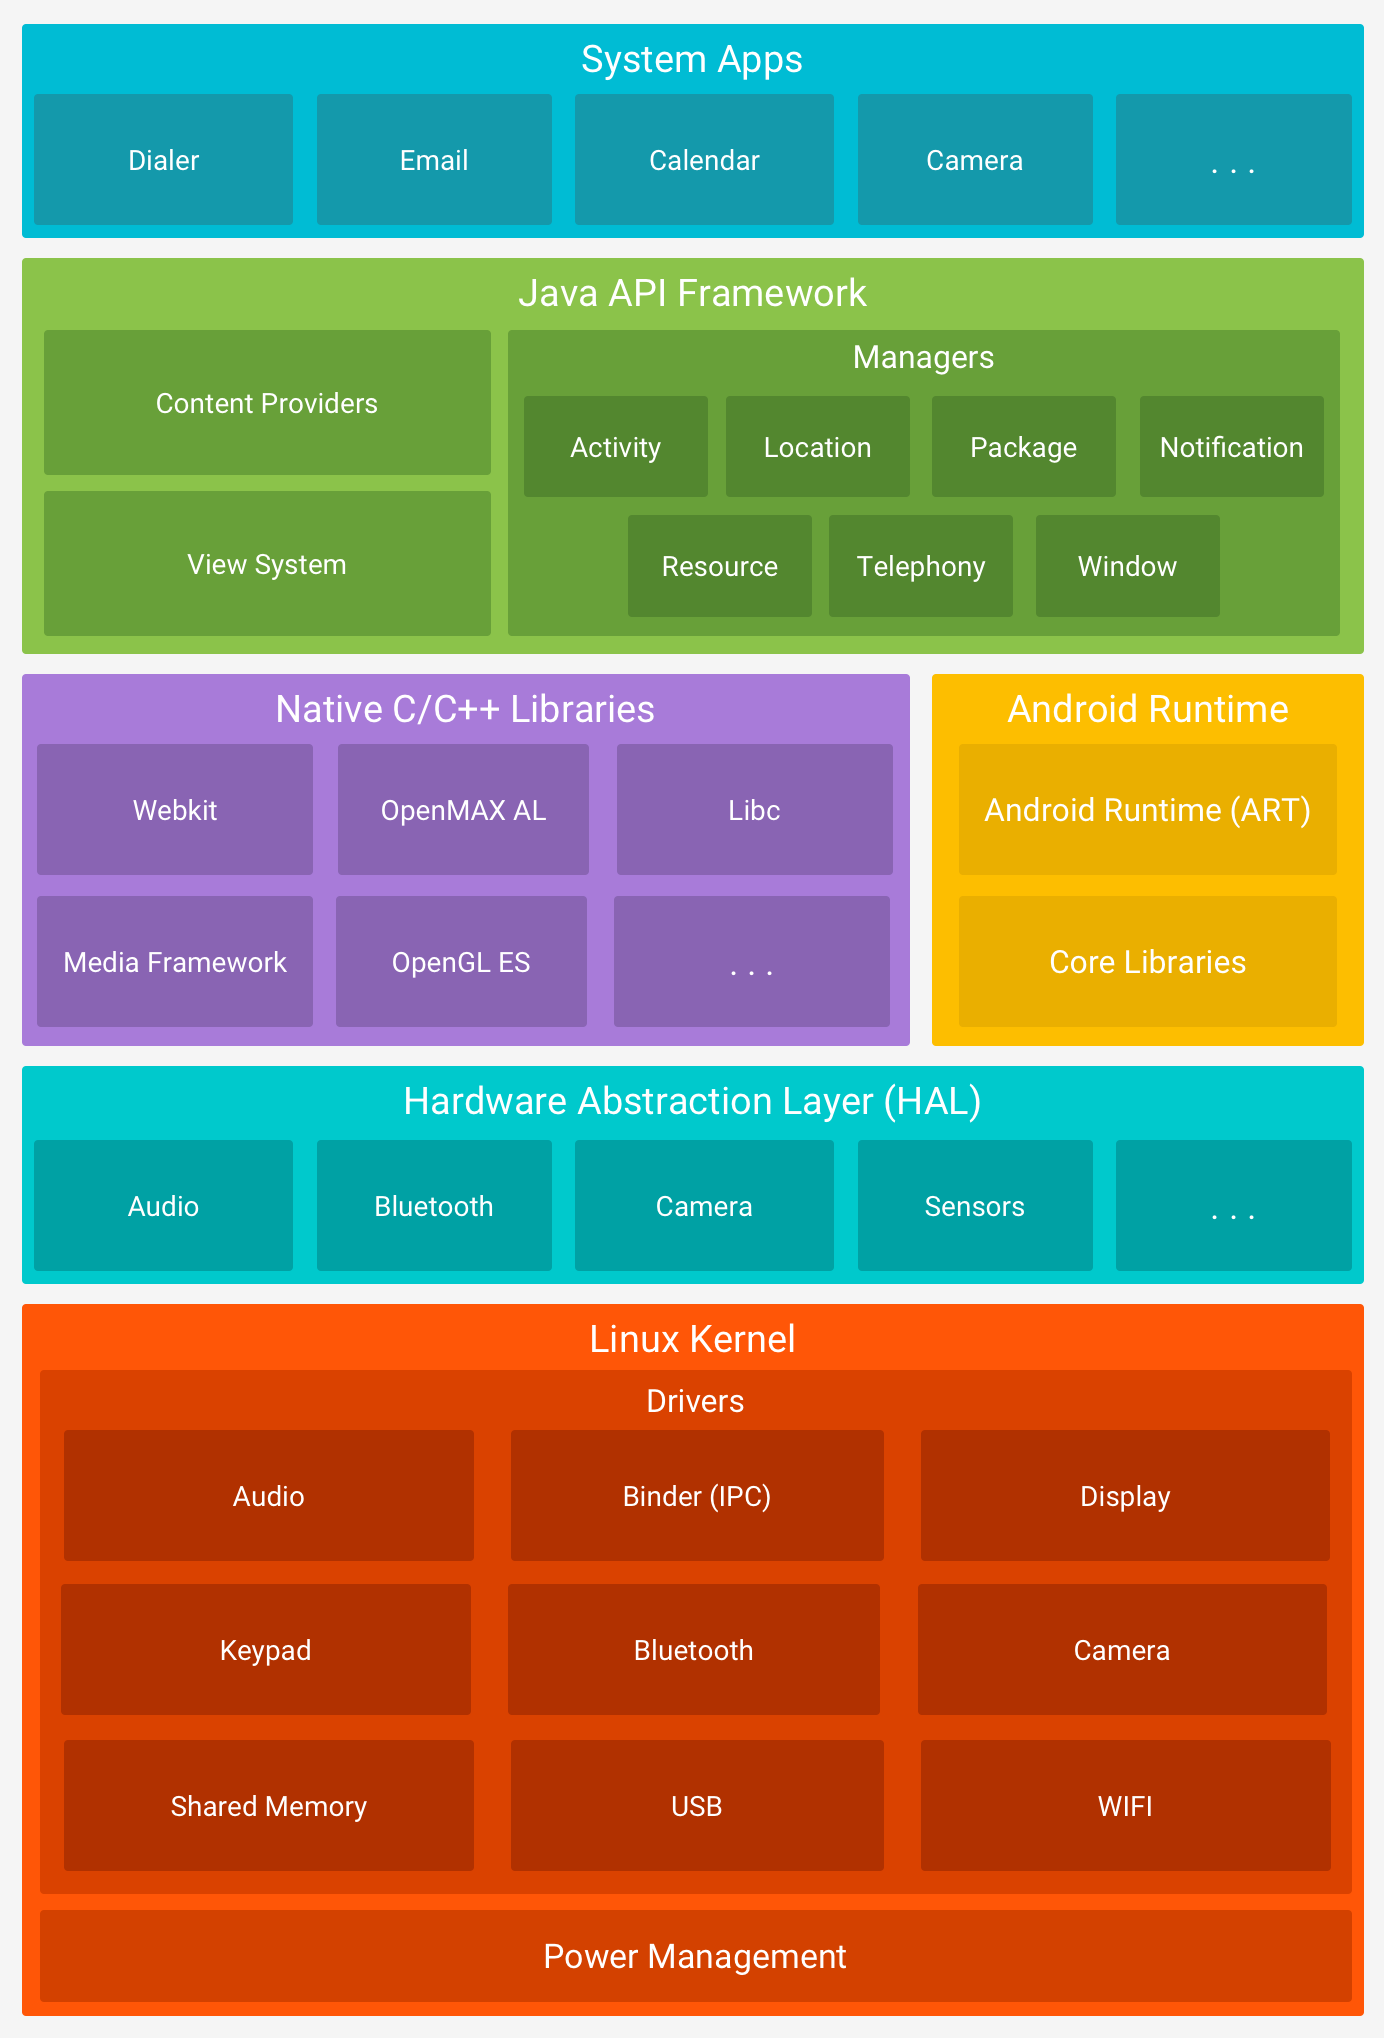
\includegraphics[width=\textwidth]{images/hello/android-stack.png}
	\label{fig:stack}
	\caption{Android is an open source, Linux-based software stack created for a wide array of devices and form factors.
			This diagram shows the major components of the Android platform. Figure from \cite{Google2017}}
\end{figure}

\begin{itemize}
	\item \textbf{Linux kernel} The Android Runtime (ART) relies on the Linux kernel for underlying functionalities such as threading and low-level memory management.
		Using a Linux kernel allows Android to take advantage of key security features!
		
		The Linux kernel provides Android with several key security features, including:	
		\begin{itemize}
			\item A user-based permissions model
			\item Process isolation
			\item Extensible mechanism for secure \textbf{I}nter-\textbf{P}rocess \textbf{C}ommunication (IPC)
			\item The ability to remove unnecessary and potentially insecure parts of the kernel
		\end{itemize}
		As a multiuser operating system, a fundamental security objective of the Linux kernel is to isolate user resources from one another.
		The Linux security philosophy is to protect user resources from one another.
		Thus, Linux:	
		\begin{itemize}
			\item Prevents user A from reading user B's files
			\item Ensures user A does not exhaust user B's memory
			\item Ensures user A does not exhaust user B's CPU resources
			\item Ensures user A does not exhaust user B's devices (e.g. telephony, GPS, Bluetooth)
		\end{itemize}		
		Moreover, the Linux Kernel  allows device manufacturers to develop hardware drivers for a well-known kernel.
		
	\item \textbf{Hardware Abstraction Layer (HAL)} This layer provides standard interfaces that expose device hardware capabilities to the higher-level Java API framework.
		The HAL consists of multiple library modules, each of which implements an interface for a specific type of hardware component, such as the camera or bluetooth module.
		When a framework API makes a call to access device hardware, the Android system loads the library module for that hardware component.
		
	\item \textbf{Android Runtime} Each app runs in its own process and with its own instance of the Android Runtime (ART).
		ART is written to run multiple virtual machines on low-memory devices by executing \textbf{DEX files}, a bytecode format designed specially for Android that's optimized for minimal memory footprint.
		It uses
		\begin{itemize}
			\item Ahead-of-time (AOT) and just-in-time (JIT) compilation \cite{}
			\item Optimized garbage collection (GC)
		\end{itemize}
		Prior to Android version 5.0 (API level 21), Dalvik was the Android runtime.
		If your app runs well on ART, then it should work on Dalvik as well, but the reverse may not be true.
		
	\item \textbf{Native C/C++ Libraries} Many core Android system components and services, such as ART and HAL, are built from code that require native libraries written in C and C++.
	
	\item \textbf{Java API Framework} The entire feature-set of the Android OS is available to you through APIs written in the Java language.
		These APIs form the building blocks you need to create Android apps by simplifying the reuse of core, modular system components and services.
		
	\item \textbf{System Apps} Android comes with a set of core apps for email, SMS messaging, calendars, internet browsing, contacts, and more.
		Apps included with the platform have no special status among the apps the user chooses to install.
		So a third-party app can become the user's default web browser, SMS messenger, or even the default keyboard (some exceptions apply, such as the system's Settings app).
\end{itemize}

\subsection{ART in detail}
\subsubsection{Android Application Development flow}
Figure \ref{fig:develop} illustrates the way an Android application is built.
This build process involves many tools and processes that convert your project into an \gls{apk}.

\begin{itemize}
	\item All resource files are combined together by Android Asset Packing Tool (AAPT).
	Resource files are audio-, video-, image-  and other asset related files.
	\item Java and Kotlin files are converted into \texttt{.class} files by the compiler.
	These \texttt{.class} files are the source for the next step in the build process.
	\item The \texttt{.class}  files are entered as input to DX tool.
	This tool converts \texttt{.class} files to \texttt{.dex} files, which include the bytecode that runs on Android devices, and everything else into compiled resources.
	\item The APK Packager combines the DEX files and compiled resources into a single APK.
	Before your app can be installed and deployed onto an Android device, however, the APK must be signed.
	\item The APK Packager signs your APK using either the debug or release keystore:
	If you are building a debug version of your app, that is, an app you intend only for testing and profiling, the packager signs your app with the debug keystore.
	Android Studio automatically configures new projects with a debug keystore.
	If you are building a release version of your app that you intend to release externally, the packager signs your app with the release keystore.
\end{itemize}


\begin{figure}[hb]
	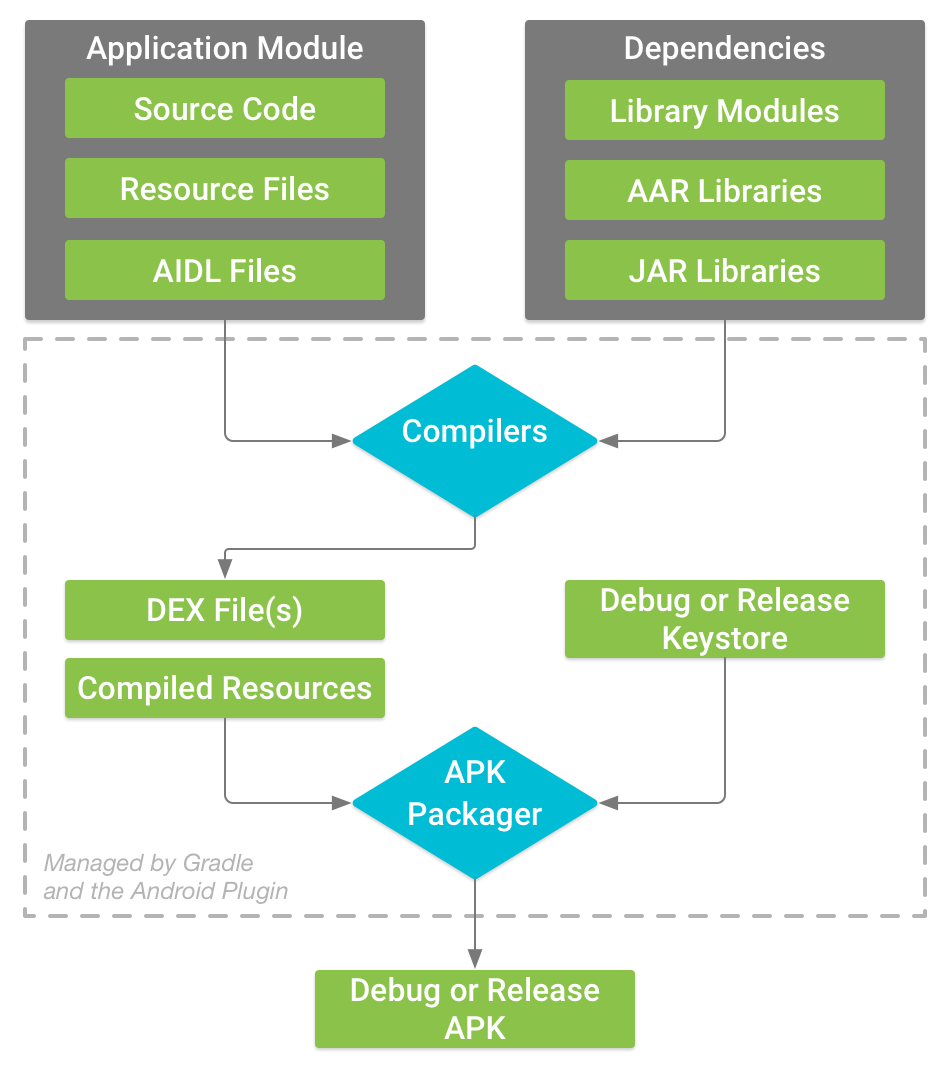
\includegraphics[width=\textwidth]{images/hello/development.png}
	\caption{The flow for building an Android application.
		Note the \gls{aidl} Figure from \cite{Developers2018build}.}
	\label{fig:develop}
\end{figure}

\subsubsection{Some words on ART \& Dalvik}
The Android runtime (ART) \cite{Android2019} is the managed runtime used by applications and some system services on Android.
ART and its predecessor Dalvik were originally created specifically for the Android project.
ART executes the Dalvik Executable format and Dex bytecode specification.

ART and Dalvik are compatible runtimes running Dex bytecode, so apps developed for Dalvik should work when running with ART.
However, some techniques that work on Dalvik do not work on ART.

The main difference between ART and Dalvik is the compilation method \cite{Vitas2013}.
Android apps are deployed in Dalvik bytecode, which is portable, unlike native code.
In order to be able to run the app on a device, the code has to be compiled to machine code.

Dalvik is based on JIT (just in time) compilation.
It means that each time you run an app, the part of the code required for its execution is going to be translated (compiled) to machine code at that moment.
As you progress through the app, additional code is going to be compiled and cached, so that the system can reuse the code while the app is running.
Since JIT compiles only a part of the code, it has a smaller memory footprint and uses less physical space on the device.

ART, on the other hand, compiles the intermediate language, Dalvik bytecode, into a system-dependent binary.
The whole code of the app will be pre-compiled during install (once), thus removing the lag that we see when we open an app on our device.
With no need for JIT compilation, the code should execute much faster.

Except for the potential speed increase, the use of ART can provide an important secondary benefit.
As ART runs app machine code directly (native execution), it doesn't hit the CPU as hard as just-in-time code compiling on Dalvik.
Less CPU usage results in less battery drain, which is a big plus for portable devices.

\section{Gradle}
TODO: stukje rond Gradle


\section{Exercises}
\begin{exercise}
	Download the latest version of Android Studio.
	Make all the necessary configurations for your operating system and create a basic project.
	You can follow the steps explained in \url{https://kotlinlang.org/docs/tutorials/kotlin-android.html}
\end{exercise}

\begin{exercise}
	Review the \texttt{build.gradle} files and try to understand what is written in there.
	What is happening in these files?
	What does the \texttt{ext.kotlin\_version} stand for?
	Is it used somewhere else? Tip: LMGTFY.
\end{exercise}

 \begin{exercise}
 	Our applications will depend on several libraries, one of them is ANKO.
	For some information on ANKO, you can read \cite{Bukros2017}.
	It is  a library that uses the power of Kotlin to simplify common tasks in Android.
	We’ll need more parts of Anko later on, but for now it’s enough to add anko-common to your project.
 \end{exercise}

\begin{exercise}
	In order to test whether everything is working fine, drag a \texttt{TextView} in the layout of a fresh Activity.
	If you have no Activity, right click your project and create one.
	We will be covering the Activity later on, for the moment don't worry about it.
	Try to alter the text at runtime by adding code in the \texttt{onCreate} method.
	Testing can be done either using the emulator or your own smartphone or tablet (if it is connected to your development machine).
\end{exercise}